\documentclass{standalone}
\usepackage{tikz}
\usetikzlibrary{patterns, positioning}

\begin{document}
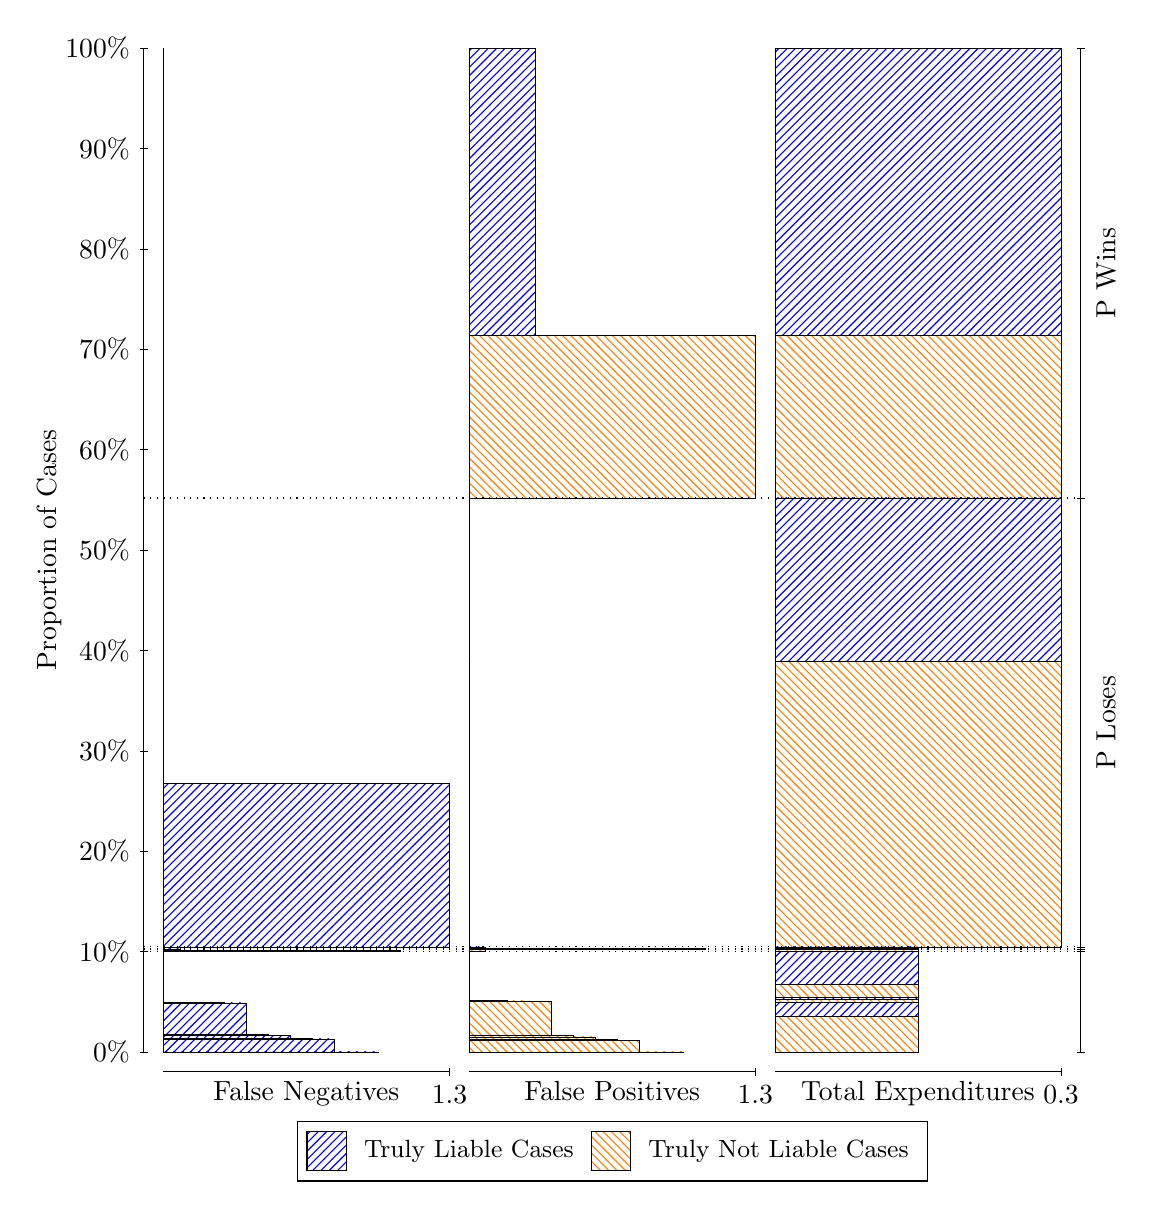
\begin{tikzpicture}
\draw[black, very thin] (1.5,1.75) -- (1.5,14.5);
\node[rotate=90, anchor=center] at (0.3, 8.125) {Proportion of Cases};
\draw[black, very thin] (1.45,1.75) -- (1.55,1.75);
\node[anchor=east] at (1.45, 1.75) {0\%};
\draw[black, very thin] (1.45,3.025) -- (1.55,3.025);
\node[anchor=east] at (1.45, 3.025) {10\%};
\draw[black, very thin] (1.45,4.3) -- (1.55,4.3);
\node[anchor=east] at (1.45, 4.3) {20\%};
\draw[black, very thin] (1.45,5.575) -- (1.55,5.575);
\node[anchor=east] at (1.45, 5.575) {30\%};
\draw[black, very thin] (1.45,6.85) -- (1.55,6.85);
\node[anchor=east] at (1.45, 6.85) {40\%};
\draw[black, very thin] (1.45,8.125) -- (1.55,8.125);
\node[anchor=east] at (1.45, 8.125) {50\%};
\draw[black, very thin] (1.45,9.4) -- (1.55,9.4);
\node[anchor=east] at (1.45, 9.4) {60\%};
\draw[black, very thin] (1.45,10.675) -- (1.55,10.675);
\node[anchor=east] at (1.45, 10.675) {70\%};
\draw[black, very thin] (1.45,11.95) -- (1.55,11.95);
\node[anchor=east] at (1.45, 11.95) {80\%};
\draw[black, very thin] (1.45,13.225) -- (1.55,13.225);
\node[anchor=east] at (1.45, 13.225) {90\%};
\draw[black, very thin] (1.45,14.5) -- (1.55,14.5);
\node[anchor=east] at (1.45, 14.5) {100\%};

\draw[black, very thin] (13.4,1.75) -- (13.4,14.5);
\draw[black, very thin] (13.35,1.75) -- (13.45,1.75);
\node[anchor=west] at (13.35, 1.75) {};
\draw[black, very thin] (13.35,3.0279) -- (13.45,3.0279);
\node[anchor=west] at (13.35, 3.0279) {};
\draw[black, very thin] (13.35,3.0577) -- (13.45,3.0577);
\node[anchor=west] at (13.35, 3.0577) {};
\draw[black, very thin] (13.35,3.0843) -- (13.45,3.0843);
\node[anchor=west] at (13.35, 3.0843) {};
\draw[black, very thin] (13.35,8.7859) -- (13.45,8.7859);
\node[anchor=west] at (13.35, 8.7859) {};
\draw[black, very thin] (13.35,14.5) -- (13.45,14.5);
\node[anchor=west] at (13.35, 14.5) {};

\draw[black, very thin, pattern color=blue, pattern=north east lines] (1.75,1.75) rectangle (4.475,1.7507);
\draw[black, very thin, pattern color=blue, pattern=north east lines] (1.75,1.7507) rectangle (4.1955,1.7519);
\draw[black, very thin, pattern color=blue, pattern=north east lines] (1.75,1.7519) rectangle (3.916,1.916);
\draw[black, very thin, pattern color=blue, pattern=north east lines] (1.75,1.916) rectangle (3.6365,1.9267);
\draw[black, very thin, pattern color=blue, pattern=north east lines] (1.75,1.9267) rectangle (3.3571,1.9579);
\draw[black, very thin, pattern color=blue, pattern=north east lines] (1.75,1.9579) rectangle (3.0776,1.9733);
\draw[black, very thin, pattern color=blue, pattern=north east lines] (1.75,1.9733) rectangle (2.7981,2.3724);
\draw[black, very thin, pattern color=blue, pattern=north east lines] (1.75,2.3724) rectangle (2.5186,2.3755);
\draw[black, very thin, pattern color=blue, pattern=north east lines] (1.75,2.3755) rectangle (2.2391,2.3775);
\draw[black, very thin, pattern color=orange, pattern=north west lines] (1.75,2.3775) rectangle (1.75,3.0279);
\draw[black, very thin, pattern color=blue, pattern=north east lines] (1.75,3.0279) rectangle (4.7545,3.0356);
\draw[black, very thin, pattern color=orange, pattern=north west lines] (1.75,3.0356) rectangle (1.75,3.0577);
\draw[black, very thin, pattern color=blue, pattern=north east lines] (1.75,3.0577) rectangle (1.9596,3.0774);
\draw[black, very thin, pattern color=orange, pattern=north west lines] (1.75,3.0774) rectangle (1.75,3.0843);
\draw[black, very thin, pattern color=blue, pattern=north east lines] (1.75,3.0843) rectangle (5.3833,5.1587);
\draw[black, very thin, pattern color=orange, pattern=north west lines] (1.75,5.1587) rectangle (1.75,8.7859);
\draw[black, very thin, pattern color=orange, pattern=north west lines] (1.75,8.7859) rectangle (1.75,10.854);
\draw[black, very thin, pattern color=blue, pattern=north east lines] (1.75,10.854) rectangle (1.75,14.5);
\draw[black, very thin, pattern color=orange, pattern=north west lines] (5.6333,1.75) rectangle (8.3583,1.7506);
\draw[black, very thin, pattern color=orange, pattern=north west lines] (5.6333,1.7506) rectangle (8.0788,1.7517);
\draw[black, very thin, pattern color=orange, pattern=north west lines] (5.6333,1.7517) rectangle (7.7994,1.8991);
\draw[black, very thin, pattern color=orange, pattern=north west lines] (5.6333,1.8991) rectangle (7.5199,1.9112);
\draw[black, very thin, pattern color=orange, pattern=north west lines] (5.6333,1.9112) rectangle (7.2404,1.9429);
\draw[black, very thin, pattern color=orange, pattern=north west lines] (5.6333,1.9429) rectangle (6.9609,1.9572);
\draw[black, very thin, pattern color=orange, pattern=north west lines] (5.6333,1.9572) rectangle (6.9609,1.9574);
\draw[black, very thin, pattern color=orange, pattern=north west lines] (5.6333,1.9574) rectangle (6.6814,2.395);
\draw[black, very thin, pattern color=orange, pattern=north west lines] (5.6333,2.395) rectangle (6.4019,2.3982);
\draw[black, very thin, pattern color=orange, pattern=north west lines] (5.6333,2.3982) rectangle (6.1224,2.4004);
\draw[black, very thin, pattern color=blue, pattern=north east lines] (5.6333,2.4004) rectangle (5.6333,3.0279);
\draw[black, very thin, pattern color=orange, pattern=north west lines] (5.6333,3.0279) rectangle (5.8429,3.05);
\draw[black, very thin, pattern color=blue, pattern=north east lines] (5.6333,3.05) rectangle (5.6333,3.0577);
\draw[black, very thin, pattern color=orange, pattern=north west lines] (5.6333,3.0577) rectangle (8.6378,3.0646);
\draw[black, very thin, pattern color=blue, pattern=north east lines] (5.6333,3.0646) rectangle (5.8429,3.0843);
\draw[black, very thin, pattern color=orange, pattern=north west lines] (5.6333,3.0843) rectangle (5.6333,6.7115);
\draw[black, very thin, pattern color=blue, pattern=north east lines] (5.6333,6.7115) rectangle (5.6333,8.7859);
\draw[black, very thin, pattern color=orange, pattern=north west lines] (5.6333,8.7859) rectangle (9.2667,10.854);
\draw[black, very thin, pattern color=blue, pattern=north east lines] (5.6333,10.854) rectangle (6.4718,14.5);
\draw[black, very thin, pattern color=orange, pattern=north west lines] (9.5167,1.75) rectangle (11.333,2.2053);
\draw[black, very thin, pattern color=blue, pattern=north east lines] (9.5167,2.2053) rectangle (11.333,2.3813);
\draw[black, very thin, pattern color=orange, pattern=north west lines] (9.5167,2.3813) rectangle (11.333,2.4151);
\draw[black, very thin, pattern color=blue, pattern=north east lines] (9.5167,2.4151) rectangle (11.333,2.447);
\draw[black, very thin, pattern color=orange, pattern=north west lines] (9.5167,2.447) rectangle (11.333,2.6083);
\draw[black, very thin, pattern color=blue, pattern=north east lines] (9.5167,2.6083) rectangle (11.333,3.0279);
\draw[black, very thin, pattern color=orange, pattern=north west lines] (9.5167,3.0279) rectangle (11.333,3.05);
\draw[black, very thin, pattern color=blue, pattern=north east lines] (9.5167,3.05) rectangle (11.333,3.0577);
\draw[black, very thin, pattern color=orange, pattern=north west lines] (9.5167,3.0577) rectangle (11.333,3.0646);
\draw[black, very thin, pattern color=blue, pattern=north east lines] (9.5167,3.0646) rectangle (11.333,3.0843);
\draw[black, very thin, pattern color=orange, pattern=north west lines] (9.5167,3.0843) rectangle (13.15,6.7115);
\draw[black, very thin, pattern color=blue, pattern=north east lines] (9.5167,6.7115) rectangle (13.15,8.7859);
\draw[black, very thin, pattern color=orange, pattern=north west lines] (9.5167,8.7859) rectangle (13.15,10.854);
\draw[black, very thin, pattern color=blue, pattern=north east lines] (9.5167,10.854) rectangle (13.15,14.5);
\draw[black, dotted] (1.5,3.0279) -- (13.4,3.0279);
\draw[black, dotted] (1.5,3.0577) -- (13.4,3.0577);
\draw[black, dotted] (1.5,3.0843) -- (13.4,3.0843);
\draw[black, dotted] (1.5,8.7859) -- (13.4,8.7859);
\draw[black, very thin] (1.75,1.5) -- (5.3833,1.5);
\node[anchor=north] at (3.5667, 1.5) {False Negatives};
\draw[black, very thin] (5.3833,1.45) -- (5.3833,1.55);
\node[anchor=north] at (5.3833, 1.45) {1.3};

\draw[black, very thin] (5.6333,1.5) -- (9.2667,1.5);
\node[anchor=north] at (7.45, 1.5) {False Positives};
\draw[black, very thin] (9.2667,1.45) -- (9.2667,1.55);
\node[anchor=north] at (9.2667, 1.45) {1.3};

\draw[black, very thin] (9.5167,1.5) -- (13.15,1.5);
\node[anchor=north] at (11.333, 1.5) {Total Expenditures};
\draw[black, very thin] (13.15,1.45) -- (13.15,1.55);
\node[anchor=north] at (13.15, 1.45) {0.3};




\node[black, centered, rotate=90] at (13.72, 5.9351) {P Loses};
\node[black, centered, rotate=90] at (13.72, 11.643) {P Wins};

\draw (7.449999999999999,1.5) node[draw=none] (baseCoordinate) {};
\begin{scope}[align=center]
        \matrix[scale=0.5, draw=black, below=0.5cm of baseCoordinate, nodes={draw}, column sep=0.1cm]{
            \node[rectangle, draw, minimum width=0.5cm, minimum height=0.5cm, pattern=north east lines, pattern color=blue] {}; &
            \node[draw=none, font=\small] (B) {Truly Liable Cases}; &
            \node[rectangle, draw, minimum width=0.5cm, minimum height=0.5cm, pattern=north west lines, pattern color=orange] {}; &
            \node[draw=none, font=\small] (B) {Truly Not Liable Cases}; \\
            };
\end{scope}

\end{tikzpicture}
\end{document}